\documentclass[12pt,a4paper]{article}
\usepackage[spanish,es-tabla]{babel}

\usepackage[utf8]{inputenc} % Escribir con acentos, ~n...
\usepackage{eurosym} % s´ımbolo del euro
\newcommand{\horrule}[1]{\rule{\linewidth}{#1}} % Create horizontal rule command with 1 argument of height
\usepackage{listings}             % Incluye el paquete listing
\usepackage[cache=false]{minted}
\usepackage{graphicx, float} %para incluir imágenes y colocarlas
\usepackage{epstopdf}

\usepackage{hyperref}
\hypersetup{
	colorlinks,
	citecolor=black,
	filecolor=black,
	linkcolor=black,
	urlcolor=black
}
\usepackage{multirow}
\usepackage{array}
\usepackage{diagbox}

\title{
\normalfont \normalsize 
\textsc{{\bf Aprendizaje Automático (2018-2019)} \\ Grado en Ingeniería Informática \\ Universidad de Granada} \\ [25pt] % Your university, school and/or department name(s)
\horrule{0.5pt} \\[0.4cm] % Thin top horizontal rule
\huge Práctica 3 \\ % The assignment title
\horrule{2pt} \\[0.5cm] % Thick bottom horizontal rule

\includegraphics{images/logo.png}	
}

\author{Antonio Jesús Heredia Castillo} % Nombre y apellidos

\date{\normalsize\today} % Incluye la fecha actual

%----------------------------------------------------------------------------------------
% DOCUMENTO
%----------------------------------------------------------------------------------------

\begin{document}

\maketitle % Muestra el Título
\newpage %inserta un salto de página
\tableofcontents % para generar el índice de contenidos
\listoffigures
\listoftables
\newpage

\section{Clasificación de dígitos}
\subsection{Comprender el problema a resolver}
La base de datos que tenemos contiene dígitos escritos a mano que se han digitalizado. Mas específicamente contiene 64 columnas por dígito sin contar la etiqueta. Los dígitos tenían un tamaño de $32\times32$ pixeles. Se realizaron agrupaciones de cuatro pixeles. Quedando 64 grupos que corresponde al numero de columnas que tenemos. En cada una de nuestras columnas tendremos la cantidad de pixeles en los que se ``ha pintado''. En la Figura \ref{fig:digitocuadricula} nos podemos hacer una idea de como se realiza las agrupaciones y que es lo que se ``cuenta''.

\begin{figure}[H]
	\centering
	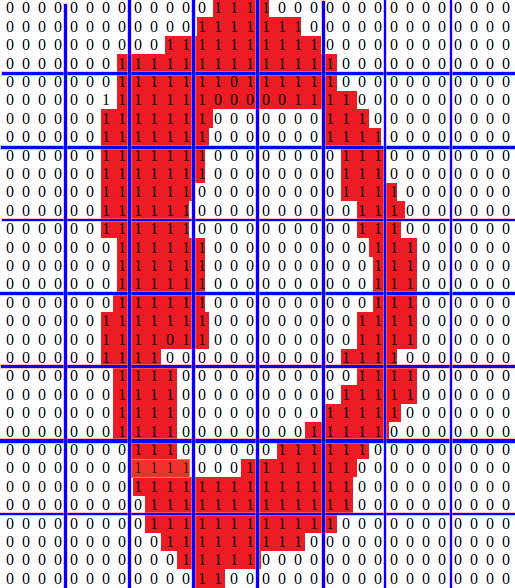
\includegraphics[scale=0.5]{images/digitoCuadricula}
	\caption[Digito cero representado con 0 y 1.]{Se puede observar las 64 agrupaciones diferentes que se realizado de los diferentes pixeles. Cada 0/1 es un pixel.}
	\label{fig:digitocuadricula}
\end{figure}

Si tenemos en cuenta las distintas agrupaciones en la $[0,0]$ tendríamos un valor de 0. En cambio en la $[0,2]$ tendríamos un valor de 6. Que en este caso es la cantidad de 1 que hay en ese grupo de pixeles. 

Aunque posteriormente tendré que unir los datos, nos los dan ya separados en entrenamiento y test. Ademas los dígitos escritos por una persona solo se encuentran en un grupo, en el de entrenamiento o en de test, pero nunca mezclados. En el grupo de entrenamiento se encuentran los dígitos de treinta personas. En el de test solamente de 13.  El conjunto de test tiene el $31.97\%$ y el de entrenamiento $68.02\%$ de los datos. \\
La etiqueta de clase es un entero entre 0 y 9. Estamos tratando un problema de clasificación de aprendizaje supervisado. Es aprendizaje supervisado ya que nos proporcionan las etiquetas.

\end{document}